\documentclass[a4j]{jarticle}
\renewcommand{\baselinestretch}{0.85}
\usepackage[top=1.5cm, bottom=1.5cm, left=1.5cm, right=1.5cm]{geometry}
\usepackage[dvipdfmx]{graphicx}
\usepackage{subcaption}
\usepackage{float}
\usepackage{booktabs}

\begin{document}

	\begin{flushright}
		MDLabグループミーティング資料\\
		25年6月3日(火)
	\end{flushright}

	\begin{center}
		{\Large	疑似ラベルを用いた自動運転のための遠赤外線画像からの物体検出}
	\end{center}

	\begin{flushright}
		{\large B4 加藤 達也}
	\end{flushright}

	\section{研究背景および目的}
	\begin{itemize}
		\item 背景: 完全自動運転の実用化に向けて技術の開発が進められており、その為に車載カメラ画像からの物体検出は重要な要素技術である。可視光画像からの物体検出は天候や時間帯によって精度が低下するので、その解決策として遠赤外線からの物体検出手法を考える。
		\item 課題:遠赤外線画像のデータセットは可視光画像のデータセットと比較して数が少ない。
		\item 目的: 遠赤外線画像を入力として低照度下でも安定的に動作する検出モデルを構築する。また、RGB画像に適応して得た検出領域を教師とするドメイン適応を用いて、遠赤外線領域における検出モデルを構築する。
	\end{itemize}
	\begin{figure}[ht]
		%複数の図を並べて出力する方法%
		\centering
		\begin{minipage}[b]{0.3\columnwidth}
			\centering
			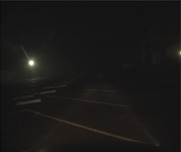
\includegraphics[height=3cm]{fig/RGB.png}%
			\caption{RGB画像}
		\end{minipage}
		\begin{minipage}[b]{0.3\columnwidth}
			\centering
			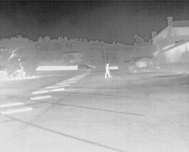
\includegraphics[height=3cm]{fig/FIR.png}%
			\caption{FIR画像}
		\end{minipage}
		\begin{minipage}[b]{0.35\columnwidth}
			\centering
			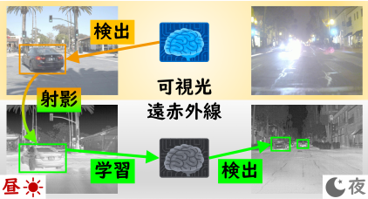
\includegraphics[height=3cm]{fig/domain_adaptation.png}%
			\caption{ドメイン適応の流れ}
		\end{minipage}
	\end{figure}
	\section{これまでの研究のまとめ}
	\begin{itemize}
		\item 谷本先輩の最終的な提案手法は以下の通りである。流れとしては図4(a)の通りである。
		\begin{enumerate}
			\item RGB画像に対して高精度な可視光モデルを用いて物体検出を行い、その結果をFIR画像に変換して疑似ラベルを生成する。
			\item 可視光モデルの出力信頼度に基づき、高信頼の検出結果のみを疑似ラベルとして使用し、誤学習を防止する。
			\item FIR画像と疑似ラベルを用いて、可視光モデルをファインチューニングし、FIR画像専用の物体検出モデルを構築する。
		\end{enumerate}
	\end{itemize}
	\begin{itemize}
		\item 損失関数のカスタマイズを行った。採用した損失関数はFocalLossとL1Loss。
		\item クラス分類とオブジェクト性にFocalLoss、バウンディングボックス回帰にSmoothL1Lossを使用した。
		\item 現在、サイズが小さいオブジェクトに対しての精度が低いため、難しいサンプルに着目し、分類性能を向上させるFocalLossを採用した。
		\item SmoothL1Lossに関してはYOLOXで中心座標と幅、高さの回帰に対してL1距離を使うことが多いため、採用した。
	\end{itemize}
	\begin{table}[htbp]
		\centering
		\begin{tabular}{|c|c|c|c|c|c|c|}
			\hline
			\textbf{Category} & \textbf{mAP} & \textbf{mAP\_50} & \textbf{mAP\_75} & \textbf{mAP\_s} & \textbf{mAP\_m} & \textbf{mAP\_l} \\
			\hline
			person & 0.039 & 0.194 & 0.001 & 0.039 & 0.079 & 0.087 \\
			car    & 0.163 & 0.490 & 0.055 & 0.039 & 0.322 & 0.644 \\
			\hline
		\end{tabular}
		\caption{各カテゴリの検出精度(例)}
	\end{table}
	\begin{itemize}
		\item mAPは閾値0.50から0.95における検出精度の平均値である。
	\end{itemize}
	\section{前回のGMからの進捗}
	\subsection{損失関数の実装について}
	\begin{itemize}
		\item configファイルはbaseファイルに上書きや追加をすることによってカスタマイズをする構造になっているが、改めてbaseファイルの方を参照して見たところ、既に損失関数は実装されていた。
		\item bboxにはIoULoss、クラス分類とオブジェクト性にCrossEntropyLossが使用されていた。
		\item この2つとも、Yoloxに最初から実装されている損失関数であったため、デフォルトの損失関数から他のカスタマイズされた損失関数に変更することによってどのように検出精度が向上するかを考えるべきであると思った。
	\end{itemize}
	\subsection{谷本先輩の修士論文時点での検出精度と現時点での検出精度の比較}
	\begin{table}[htbp]
	\centering
	\caption{谷本先輩の検出精度($\theta_{\mathrm{det}}=0.50$,lr=0.01),best\_epoc=100}
		\begin{tabular}{lcccccc}
			\hline
			\textbf{category} & \textbf{mAP} & \textbf{mAP\_50} & \textbf{mAP\_75} & \textbf{mAP\_s} & \textbf{mAP\_m} & \textbf{mAP\_l} \\
			\hline
			person & 0.024 & 0.108 & 0.001 & 0.027 & 0.072 & 0.100 \\
			car    & 0.299 & 0.567 & 0.293 & 0.119 & 0.553 & 0.758 \\
			\hline
		\end{tabular}
	\end{table}

	\begin{table}[htbp]
	\centering
	\caption{私の検出精度($\theta_{\mathrm{det}}=0.70$,lr=0.00125),best\_epoc=10}
		\begin{tabular}{lcccccc}
			\hline
			\textbf{category} & \textbf{mAP} & \textbf{mAP\_50} & \textbf{mAP\_75} & \textbf{mAP\_s} & \textbf{mAP\_m} & \textbf{mAP\_l} \\
			\hline
			person & 0.069 & 0.236 & 0.210 & 0.058 &0.167 & 0.118 \\
			car    & 0.294 & 0.638 & 0.253 & 0.143 & 0.532 & 0.761 \\
			\hline
		\end{tabular}
	\end{table}

	\begin{itemize}
		\item $\theta_{\mathrm{det}}$は信頼度であり、信頼度以上のものが疑似ラベルとして使用される。
		\item 手順は全く変わっておらず、RGB画像を元に疑似ラベルを作成→SAM2でのアノテーション→学習・検証である。違いとしては損失関数の変更と、細かいパラメータの変更である。
		\item mAPが上がった原因としては、クラス分類の損失関数として設定しているFocalLossにおいて、バランス係数(alpha)をpersonとcarそれぞれに0.60と0.40と設定してクラス不均衡を減そうとしたことである。また、信頼度を0.50から0.70へ変更した。
		\item しかし、FocalLossの特性上の問題か、検出が難しいpersonに重みをおいているので、carの検出精度が僅かに下がっている。
	\end{itemize}
	\begin{equation}
		FL (P_t) = - \alpha _ t(1 - p_t)^ \gamma log(p_t)
	\end{equation}
	\begin{itemize}
		\item (1)はFocalLossの数式であり、$\alpha$はバランス係数であり、クラス間に不均衡がある場合に少ないクラスに対して損失の重みを大きくするために使う。\cite{FocalLoss}
		\item $\gamma$は困難サンプルに集中するためのパラメータであり、判別が容易であるサンプルの影響を抑え、難しいサンプルに注目するための関数である。
		\item どちらも大きい数値であればあるほど影響は大きい。
	\end{itemize}
		\begin{itemize}
		\item またバッチサイズがYolox\_sとYolox\_xでそれぞれ16と8であるが、学習率が一律で0.01になっていたので修正した。
		\item Yolox\_sは0.0025、Yolox\_xは0.00125とした。
		\item 根拠としてはYOLOX: Exceeding YOLO Series in 2021において(2)で学習率を定めていたことからである。\cite{learning_rate}
	\end{itemize}
	\begin{equation}
		lr_{actually} = lr × BatchSize / 64 (lr=0.01)
	\end{equation}
	\subsection{ITSミーティングについて}
	\begin{itemize}
		\item 愛知工科大学の久徳先生との毎週月曜日に行われるITSミーティングにおいて、ご指摘をいただいた。
		\item 学習率は一つの数式で決まるものではないので、繰り返し実験して自分の環境にあった学習率を模索するべき。
		\item 損失関数については既存の損失関数はそれぞれ想定された使い方が存在するので、それに従って適した損失関数を各所に実装する。また、数値だけではなく描画されるものも見て損失関数の傾向を掴む。
		\item 既存の損失関数でも良いが、谷本先輩は独自の計算での損失関数の作成を目指していた。
	\end{itemize}
	\section{今後の課題\&スケジュール}
		\begin{itemize}
			\item FLIRのバージョンアップをする。
			\item 損失関数に関する理解を深め、より良い検出精度を目指す。できれば独自の計算で損失関数を作成したい。
		\end{itemize}

\begin{thebibliography}{10}
	\bibitem{FocalLoss}Tsung-Yi Lin, Priya Goyal, Ross Girshick, Kaiming He, Piotr Dollár Focal Loss for Dense Object Detection (7 Feb 2018)
	\bibitem{learning_rate}Zheng Ge,Songtao Liu,Feng Wang,Zeming Li,Jian Sun YOLOX: Exceeding YOLO Series in 2021 (6 Aug 2021)
\end{thebibliography}
\end{document}
